\documentclass[tikz,border=5mm]{standalone}
\usetikzlibrary{positioning, shapes, fit, arrows.meta, calc, backgrounds, matrix, decorations.pathreplacing}
\usepackage{amssymb}

\definecolor{kellygreen}{rgb}{0.15, 0.50, 0.12}
\definecolor{darkgreen}{rgb}{0.04, 0.3, 0.03}
\definecolor{darkgray}{rgb}{0.30, 0.30, 0.30}
\definecolor{gray}{rgb}{0.53, 0.53, 0.53}
\definecolor{slate}{rgb}{0.094,0.094,0.094}
\definecolor{cobalt}{rgb}{0.244,0.364,0.972}

\usepackage[scaled]{helvet}
\renewcommand\familydefault{\sfdefault}
\usepackage[T1]{fontenc}

\begin{document}
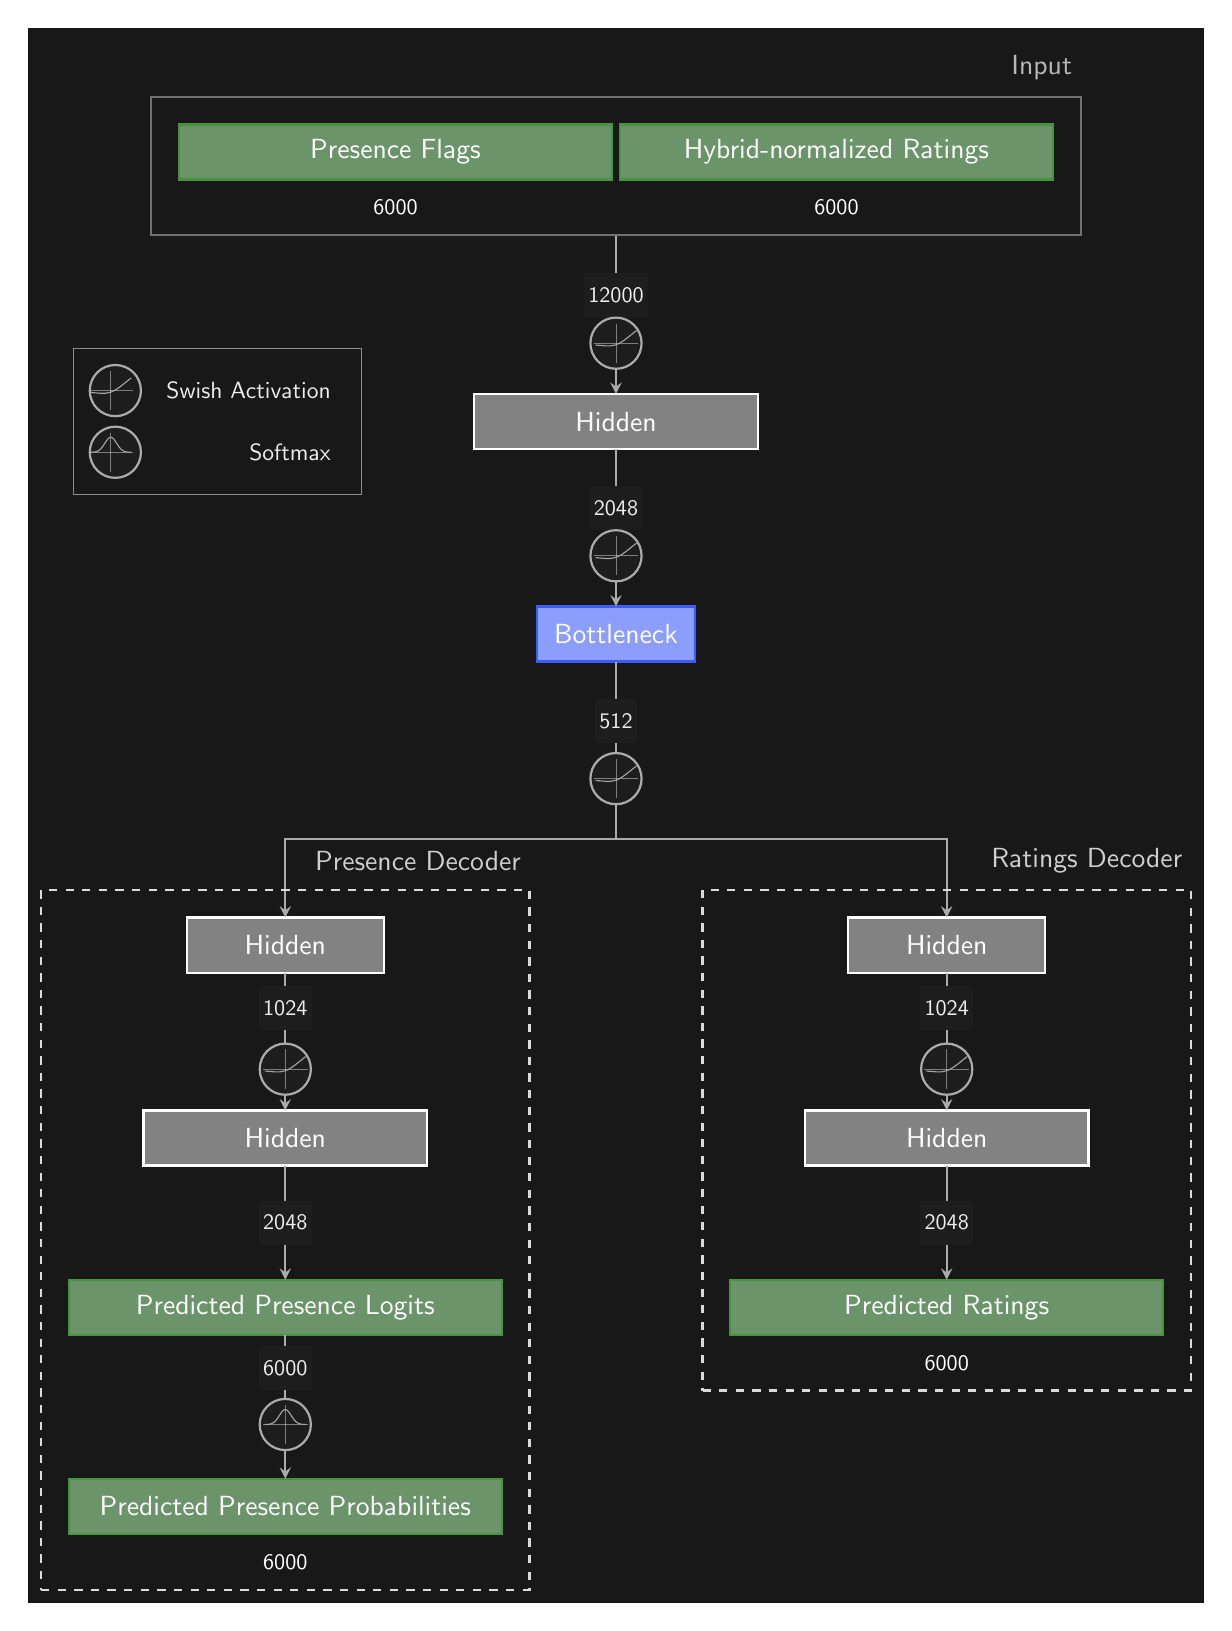
\begin{tikzpicture}[
    background rectangle/.style={fill=slate},
    show background rectangle,
    node distance=1.45cm and 1cm,
    every node/.style={rectangle, align=center, color=white, text=white, fill=none, minimum height=0.7cm},
    layer/.style={
        rectangle,
        draw,
        thick,
        fill=darkgray!70,
        inner sep=2pt,
        outer sep=0pt
    },
    io/.style={
        rectangle,
        draw=kellygreen!85,
        thick,
        fill=darkgreen!60,
        inner sep=5pt,
        outer sep=0pt
    },
    dimlbl/.style={
        midway,
        fill=slate!98,
        inner sep=2pt,
        scale=0.8,
        text=gray!15,
    },
    extlbl/.style={
      fill=slate!98,
      inner sep=2pt,
      scale=0.8,
      text=gray!15,
    },
    arr/.style={
        ->,
        thick,
        >=stealth,
        draw=gray!70,
        gray!70
    },
    headless/.style={
        thick,
        draw=gray!70
    },
    % =======================
    % Small activation icons
    % =======================
    actBase/.style={
        circle,
        draw=gray!70,
        thick,
        fill=slate!98,
        minimum size=6.5mm,
        inner sep=0pt
    },
    actSwish/.style={
      actBase,
      path picture={
        \begin{scope}
          \clip (path picture bounding box.south west) rectangle (path picture bounding box.north east);
          \begin{scope}[shift={(0mm,-0.200mm)}, yscale=2, shift={(0mm,0.200mm)}]
            \draw[-, gray!40, line width=0.25pt, opacity=0.55]
              (-2.85mm, 0mm) -- (2.85mm, 0mm);
            \draw[-, gray!40, line width=0.25pt, opacity=0.55]
              (0.000mm, -2.5mm) -- (0.000mm, 2.5mm);
            \draw[-, gray!75, line width=0.4pt]
              (-2.600mm, -0.233mm)
                .. controls (-1.733mm, -0.265mm) and (-0.867mm, -0.505mm) ..
              ( 0.000mm, -0.200mm)
                .. controls ( 0.867mm,  0.105mm) and ( 1.733mm,  0.957mm) ..
              ( 2.600mm,  1.600mm);
          \end{scope}
        \end{scope}
      }
    },
    % "Gaussian-like" curve (softmax icon) with the same axis styling as swish.
    % Control points chosen to closely match a bell curve in this tiny viewport.
    actGauss/.style={
      actBase,
      path picture={
        \begin{scope}
          \clip (path picture bounding box.south west) rectangle (path picture bounding box.north east);
          \begin{scope}[shift={(0mm,-0.200mm)}, yscale=2, shift={(0mm,0.200mm)}]
            \draw[-, gray!40, line width=0.25pt, opacity=0.55]
              (-2.85mm, 0mm) -- (2.85mm, 0mm);
            \draw[-, gray!40, line width=0.25pt, opacity=0.55]
              (0.000mm, -2.5mm) -- (0.000mm, 2.5mm);
            % bell curve (Gaussian-like) drawn by plotting an analytic function
            \draw[-, gray!75, line width=0.4pt, smooth]
              plot[domain=-2.6:2.6, samples=60]
                ({\x*1mm}, {1.9*exp(-(\x/1.05)^2)*1mm});
          \end{scope}
        \end{scope}
      }
    },
]

% =======================
% Sizing
% =======================
\pgfmathsetmacro{\wInputSplit}{5.5cm}
\pgfmathsetmacro{\wEncoder}{3.6cm}
\pgfmathsetmacro{\wBottleneck}{2.0cm}
\pgfmathsetmacro{\wDecMid}{2.5cm}
\pgfmathsetmacro{\wDecFinal}{3.6cm}
\pgfmathsetmacro{\headSep}{4.2cm}

% =======================
% Top Section: Inputs
% =======================
\node[io, minimum width=\wInputSplit] (in_pres) {Presence Flags};
\node[below=2pt of in_pres, scale=0.8] (in_pres_label) {6000};

\node[io, right=0.1cm of in_pres, minimum width=\wInputSplit] (in_rate) {Hybrid-normalized Ratings};
\node[below=1pt of in_rate, scale=0.45] (in_rate_label_anchor) {};
\node[below=2pt of in_rate, scale=0.8] (in_rate_label) {6000};

\node[draw=darkgray!80, thick, fit=(in_pres)(in_rate)(in_rate_label_anchor), inner sep=10pt,
      label={[gray!60, anchor=south east]north east:Input}] (input_container) {};

\coordinate[below=1cm of input_container] (merge_point);

% =======================
% Middle Section: Encoder & Bottleneck
% =======================
\node[layer, below=1.0cm of merge_point, minimum width=\wEncoder] (encoder) {Hidden};

\node[layer, below=2.0cm of encoder, minimum width=\wBottleneck,
      fill=cobalt!60, draw=cobalt] (bottleneck) {Bottleneck};

% =======================
% Bottom Section: Decoder Branches
% =======================
% Make this segment longer to avoid the swish+dim overlap on the fan-out stem.
\coordinate[below=2.25cm of bottleneck] (split_point);

\node[layer, below=1.0cm of split_point, xshift=-\headSep, anchor=north, minimum width=\wDecMid] (dec1_h1) {Hidden};
\node[layer, below=1.75cm of dec1_h1, minimum width=\wDecFinal] (dec1_h2) {Hidden}; % <- was below=of
\node[io, below=of dec1_h2, minimum width=\wInputSplit] (out_pres) {Predicted Presence Logits};
\node[below=1pt of out_pres, scale=0.45] (out_pres_label_anchor) {};

\node[layer, below=1.0cm of split_point, xshift=\headSep, anchor=north, minimum width=\wDecMid] (dec2_h1) {Hidden};
\node[layer, below=1.75cm of dec2_h1, minimum width=\wDecFinal] (dec2_h2) {Hidden}; % <- was below=of
\node[io, below=of dec2_h2, minimum width=\wInputSplit] (out_rate) {Predicted Ratings};
\node[below=2pt of out_rate, scale=0.8] (out_rate_label) {6000};
\node[below=1pt of out_rate, scale=0.45] (out_rate_label_anchor) {};

% =======================
% Legend (top-left, vertically ~aligned with encoder)
% =======================
\matrix (legend_mat) [
  matrix of nodes,
  nodes={anchor=east, text=gray!15},
  row sep=3pt,
  column sep=6pt,
  anchor=east
] at ([xshift=-1.5cm]encoder.west) {
  |[actSwish]| {} & |[scale=0.85]| {Swish Activation} \\
  |[actGauss]| {} & |[scale=0.85]| {Softmax} \\
};
\node[draw=gray!95, fit=(legend_mat), inner sep=2pt] (legend_box) {};

% =======================
% Connections + Swish markers (stacked vertically)
% =======================
% Slightly larger y-shifts so the dim + icon never touch.
\draw[arr] (input_container) --
  node[pos=0.52, dimlbl, yshift=9pt] {12000}
  node[pos=0.52, actSwish, yshift=-9pt] {}
  (encoder);

\draw[arr] (encoder) --
  node[pos=0.52, dimlbl, yshift=9pt] {2048}
  node[pos=0.52, actSwish, yshift=-9pt] {}
  (bottleneck);

% Single arrow out of bottleneck with the ONLY decoder-side swish, then split
\draw[headless] (bottleneck.south) --
  node[pos=0.52, dimlbl, yshift=13pt] {512}
  node[pos=0.52, actSwish, yshift=-9pt] {}
  (split_point);

% --- add Swish markers between the hidden layers in each decoder head ---
\draw[arr] (split_point) -| (dec1_h1);
\draw[arr] (dec1_h1) --
  node[pos=0.52, dimlbl, yshift=15pt] {1024}
  node[pos=0.52, actSwish, yshift=-9pt] {}
  (dec1_h2);
\draw[arr] (dec1_h2) -- node[dimlbl] {2048} (out_pres);

\draw[arr] (split_point) -| (dec2_h1);
\draw[arr] (dec2_h1) --
  node[pos=0.52, dimlbl, yshift=15pt] {1024}
  node[pos=0.52, actSwish, yshift=-9pt] {}
  (dec2_h2);
\draw[arr] (dec2_h2) -- node[dimlbl] {2048} (out_rate);

% =======================
% Softmax (moved beneath presence logits) + probabilities output
% =======================
\node[actGauss, below=0.8cm of out_pres.south] (softmax_icon) {};
%\node[above=1pt of softmax_icon, scale=0.75, text=gray!25] {Softmax};
\draw[headless] (out_pres.south) -- (softmax_icon.north);

\node[io, below=0.35cm of softmax_icon.south, minimum width=\wInputSplit] (out_pres_prob) {Predicted Presence Probabilities};
\node[below=2pt of out_pres_prob, scale=0.8] (out_pres_prob_label) {6000};
\node[below=1pt of out_pres_prob, scale=0.45] (out_pres_prob_label_anchor) {};

\draw[arr] (softmax_icon.south) -- (out_pres_prob.north);

\node[fill=slate!98, inner sep=2pt, text=gray!15, below=4pt of out_pres, extlbl] (out_pres_label) {6000};

% =======================
% Decoder containers (presence now taller than ratings)
% =======================
\node[draw=gray!30, dashed, thick,
      fit=(dec1_h1)(out_pres)(out_pres_label_anchor)(softmax_icon)(out_pres_prob)(out_pres_prob_label_anchor),
      inner sep=10pt,
      label={[gray!40, anchor=south east]north east:Presence Decoder}] (dec1_container) {};

\node[draw=gray!30, dashed, thick,
      fit=(dec2_h1)(out_rate)(out_rate_label_anchor),
      inner sep=10pt,
      label={[gray!40, anchor=south east]north east:Ratings Decoder}] (dec2_container) {};

\end{tikzpicture}
\end{document}
